\documentclass[12pt,a4paper]{article}

\usepackage[utf8]{inputenc}
\usepackage[T1]{fontenc}
\usepackage{geometry}
\usepackage{amsmath}
\usepackage{enumitem}
\usepackage{tikz}
\usepackage{xcolor}
\usepackage{tcolorbox}
\usepackage{graphicx}
\usepackage{float}

\usetikzlibrary{
    positioning,
    arrows.meta,
    shapes.geometric
}

\geometry{margin=2.5cm}

% Colours
\definecolor{atcnavy}{RGB}{20,45,80}
\definecolor{atclightblue}{RGB}{190,215,240}
\definecolor{atcamber}{RGB}{220,150,30}
\definecolor{atcred}{RGB}{190,45,45}
\definecolor{atcgreen}{RGB}{40,130,75}
\definecolor{atcslate}{RGB}{90,100,115}

% Custom box
\newtcolorbox{successbox}[1][]{
    colback=green!5,
    colframe=green!50!black,
    title=#1,
    fonttitle=\bfseries
}

\begin{document}
% =========================================================================
\section{Agent Selection \& Multi-Crew Architecture}
% =========================================================================

\subsection{Architectural Addition: Crew 4 (Safety Validation \& Quality Assurance)}

The assignment includes four main crews: \textit{Data Management}, \textit{Surveillance \& Conflict}, \textit{Tactical Resolution}, and \textit{Reporting}. We have added a fifth crew called the \textbf{Safety Validation \& Quality Assurance Crew}.

\begin{successbox}[Domain Justification for Additional Crew ]
In Air Traffic Control Systems, changing the route of Aircraft $A$ to avoid Aircraft $B$ could create a new conflict with another aircraft, such as Aircraft $C$. It could also cause too many aircraft to enter the same airspace sector.

Having a separate safety crew means that every updated flight plan is checked again before final approval. This helps make sure that the new routes are safe and do not create any other conflicts.
\end{successbox}

\begin{figure}[htbp]
\centering

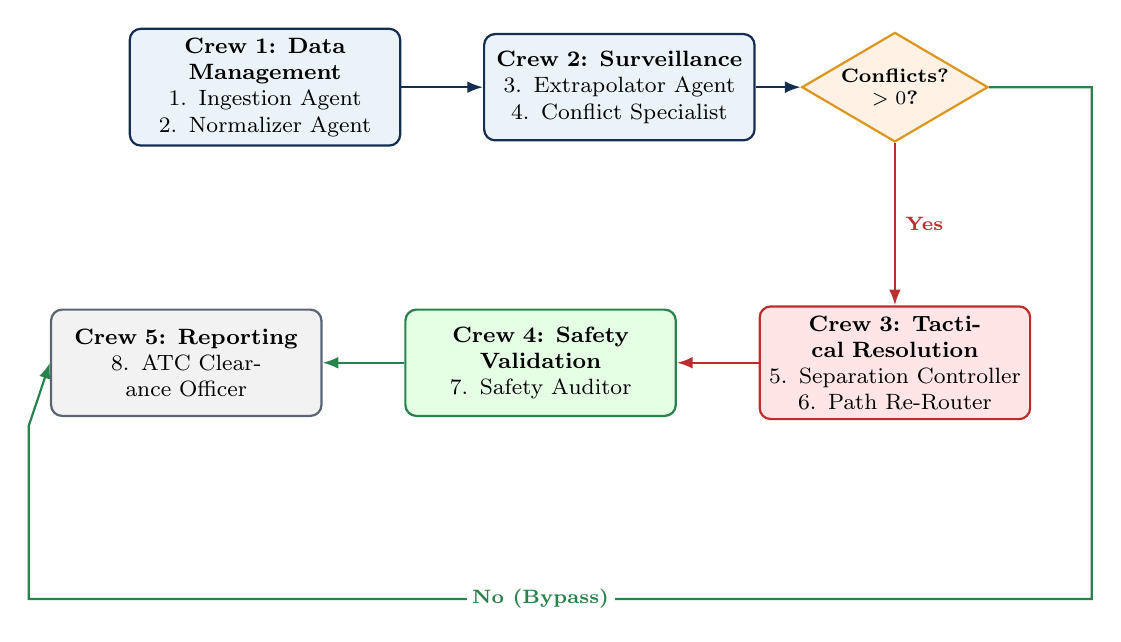
\begin{tikzpicture}[
    crewbox/.style={
        rectangle,
        rounded corners,
        draw=atcnavy,
        fill=atclightblue!30,
        thick,
        text width=3.2cm,
        minimum height=1.35cm,
        align=center,
        font=\footnotesize
    },
    routerbox/.style={
        diamond,
        draw=atcamber,
        fill=orange!10,
        thick,
        aspect=1.7,
        align=center,
        font=\scriptsize\bfseries,
        inner sep=1pt
    },
    arrow/.style={
        -{Latex[length=2mm]},
        thick,
        draw=atcnavy
    }
]

% TOP ROW
\node[crewbox] (c1) at (0,2.5) {
    \textbf{Crew 1: Data Management}\\
    1. Ingestion Agent\\
    2. Normalizer Agent
};

\node[crewbox] (c2) at (4.5,2.5) {
    \textbf{Crew 2: Surveillance}\\
    3. Extrapolator Agent\\
    4. Conflict Specialist
};

\node[routerbox] (rtr) at (8,2.5) {
    Conflicts?\\
    $>0$?
};

% BOTTOM ROW
\node[crewbox, fill=red!10, draw=atcred] (c3) at (8,-1) {
    \textbf{Crew 3: Tactical Resolution}\\
    5. Separation Controller\\
    6. Path Re-Router
};

\node[crewbox, fill=green!10, draw=atcgreen] (c4) at (3.5,-1) {
    \textbf{Crew 4: Safety Validation}\\
    7. Safety Auditor
};

\node[crewbox, fill=gray!10, draw=atcslate] (c5) at (-1,-1) {
    \textbf{Crew 5: Reporting}\\
    8. ATC Clearance Officer
};

% MAIN FLOW
\draw[arrow] (c1.east) -- (c2.west);
\draw[arrow] (c2.east) -- (rtr.west);

% YES: Tactical resolution
\draw[arrow, draw=atcred]
    (rtr.south) -- node[right, font=\scriptsize\bfseries, text=atcred]
    {Yes} (c3.north);

% Tactical resolution -> Safety validation
\draw[arrow, draw=atcred]
    (c3.west) -- (c4.east);

% Safety validation -> Reporting
\draw[arrow, draw=atcgreen]
    (c4.west) -- (c5.east);



% NO: Bypass route completely outside the crew boxes

\draw[
    -{Latex[length=2mm]},
    thick,
    draw=atcgreen
]
(rtr.east)
-- (10.5,2.5)
-- (10.5,-4.0)
-- (-3.0,-4.0)
-- (-3.0,-1.8)
-- (c5.west);

\node[
    font=\scriptsize\bfseries,
    text=atcgreen,
    fill=white,
    inner sep=2pt
] at (3.5,-4.0) {No (Bypass)};
\end{tikzpicture}

\caption{CrewAI Multi-Agent System Architecture with Dynamic Routing and Five Crews.}
\end{figure}


\subsection{Detailed Agent Specifications}

\subsubsection{Crew 1: Data Management Crew}

\begin{itemize}[leftmargin=*]
    \item \textbf{Agent 1: Airspace \& Topology Ingestion Specialist}
\begin{itemize}
    \item \textit{Role:} Aviation GIS and Network Specialist.
    \item \textit{Main Task:} Read the GraphML network, check that waypoint coordinates are correct, and make sure the airways are connected properly.
    \item \textit{Tools:} \texttt{GraphMLAirspaceParserTool}, \texttt{AirspaceConnectivityValidatorTool}.
\end{itemize}

    \item \textbf{Agent 2: Flight Data Normalization Officer}
\begin{itemize}
    \item \textit{Role:} Air Traffic Data Engineer.
    \item \textit{Main Task:} Match the aircraft specifications in the JSON file with the flight schedules, make sure the timestamps are in the correct order, and create standard Pydantic \texttt{FlightPlanModel} instances.
    \item \textit{Tools:} \texttt{FlightPlanNormalizerTool}, \texttt{JSONSchemaValidatorTool}.
\end{itemize}
\end{itemize}


\subsubsection{Crew 2: Surveillance \& Conflict Crew}

\begin{itemize}[leftmargin=*]
    \item \textbf{Agent 3: Radar Surveillance \& Trajectory Extrapolator}
\begin{itemize}
    \item \textit{Role:} 4D Airspace Tracking Specialist.
    \item \textit{Main Task:} Estimate the future 4D flight paths $(x(t), y(t), z(t))$ for all aircraft by calculating their positions between waypoints using their assigned cruising speeds.
    \item \textit{Tools:} \texttt{TrajectoryExtrapolatorTool}.
\end{itemize}

    \item \textbf{Agent 4: Separation \& Conflict Detection Specialist}
\begin{itemize}
    \item \textit{Role:} Tactical Radar Safety Analyst.
    \item \textit{Main Task:} Compare the flight paths of aircraft in pairs to find conflicts where the horizontal distance is less than $5\text{ NM}$ or the vertical distance is less than $1,000\text{ ft}$. Also, calculate the Closest Point of Approach (CPA) and the level of risk.
    \item \textit{Tools:} \texttt{SeparationMinimaCheckerTool}, \texttt{ConflictSeverityClassifierTool}.
\end{itemize}
\end{itemize}


\subsubsection{Crew 3: Tactical Resolution Crew}

\begin{itemize}[leftmargin=*]
    \item \textbf{Agent 5: Tactical Separation Controller}
    \begin{itemize}
        \item \textit{Role:} Lead Tactical Air Traffic Controller.
        \item \textit{Main Task:} Choose which aircraft should change its flight path to avoid a conflict. This agent can change the Flight Level (e.g. FL350 to FL330) or adjust the aircraft's speed by following ICAO rules.
        \item \textit{Tools:} \texttt{AltitudeLevelAllocatorTool}, \texttt{ManeuverCostEvaluatorTool}.
    \end{itemize}

    \item \textbf{Agent 6: Flight Path Re-Router}
    \begin{itemize}
        \item \textit{Role:} Airspace Navigation and Path Revision Specialist.
        \item \textit{Main Task:} Find an alternative route using other GraphML airway nodes when changing the aircraft's altitude is not enough to avoid the conflict.
        \item \textit{Tools:} \texttt{AirspaceGraphRoutingTool}, \texttt{FlightPlanModifierTool}.
    \end{itemize}
\end{itemize}


\subsubsection{Crew 4: Safety Validation \& Quality Assurance Crew (Additional Crew)}

\begin{itemize}[leftmargin=*]
    \item \textbf{Agent 7: Airspace Safety \& Compliance Auditor}
    \begin{itemize}
        \item \textit{Role:} Independent Airspace Safety Inspector.
        \item \textit{Main Task:} Check the proposed flight plans again against all aircraft to find any new conflicts, make sure sector capacity limits are followed, and give Safety Clearances.
        \item \textit{Tools:} \texttt{SecondaryConflictVerifierTool}, \texttt{ATCComplianceAuditTool}.
    \end{itemize}
\end{itemize}


\subsubsection{Crew 5: Reporting Crew}
\begin{itemize}[leftmargin=*]
    \item \textbf{Agent 8: ATC Clearance \& Reporting Officer}
    \begin{itemize}
        \item \textit{Role:} Chief Documentation \& Clearance Officer.
        \item \textit{Main Task:} Combine the initial airspace situation, conflict logs, actions taken to resolve conflicts, and safety audit certificates into a complete Markdown ATC report.
        \item \textit{Tools:} \texttt{MarkdownReportGeneratorTool}, \texttt{ClearanceSummaryFormatterTool}.
    \end{itemize}
\end{itemize}

\end{document}